\documentclass[10pt,a4paper]{report}
\usepackage{fancyhdr}
\usepackage{lastpage}
\usepackage{graphicx}
\usepackage{listings}
\graphicspath{{./images/}}

% Title Page
\title{Third Year Project Progress Report}
\date{18 November 2019}

\pagestyle{fancy}
\fancyhf{} % clear all fields

\fancyhead[R]{Toby Lawrance, 1731636, \thepage / \pageref{LastPage}}
\renewcommand{\headrulewidth}{0pt}

\begin{document}
\maketitle
\section*{Project Introduction/Specification}
	\subsection*{Statement}
		\subsubsection*{In Short:}
			Implementing Computer Vision algorithms to allow for robot navigation using the camera feed as the primary perception.
		\subsubsection*{Aims:}
			The aim of this project is to utilise the camera more efficiently as cameras are typically cheap sensors and this helps make robotics more affordable as a discipline, or at least to provide additional ways to aid internal sensor data and provide additional data points of belief in the robot's current pose.
		\subsubsection*{Objectives:}
			\begin{enumerate}
				\item Move towards an object that is recognised in the environment. 
				\item Acknowledge obstacles in the environment and attempt to avoid them.
				\item Acknowledge more natural obstacles.
				\item Use the camera feed to aid with pose estimation.
			\end{enumerate}
\section*{Progress made so far}
	\subsection*{TurtleBot3}
		\subsection*{The TurtleBot3}
			The department has kindly allowed me the use of a TurtleBot3 for this project which upon receiving, I promptly built: \\
			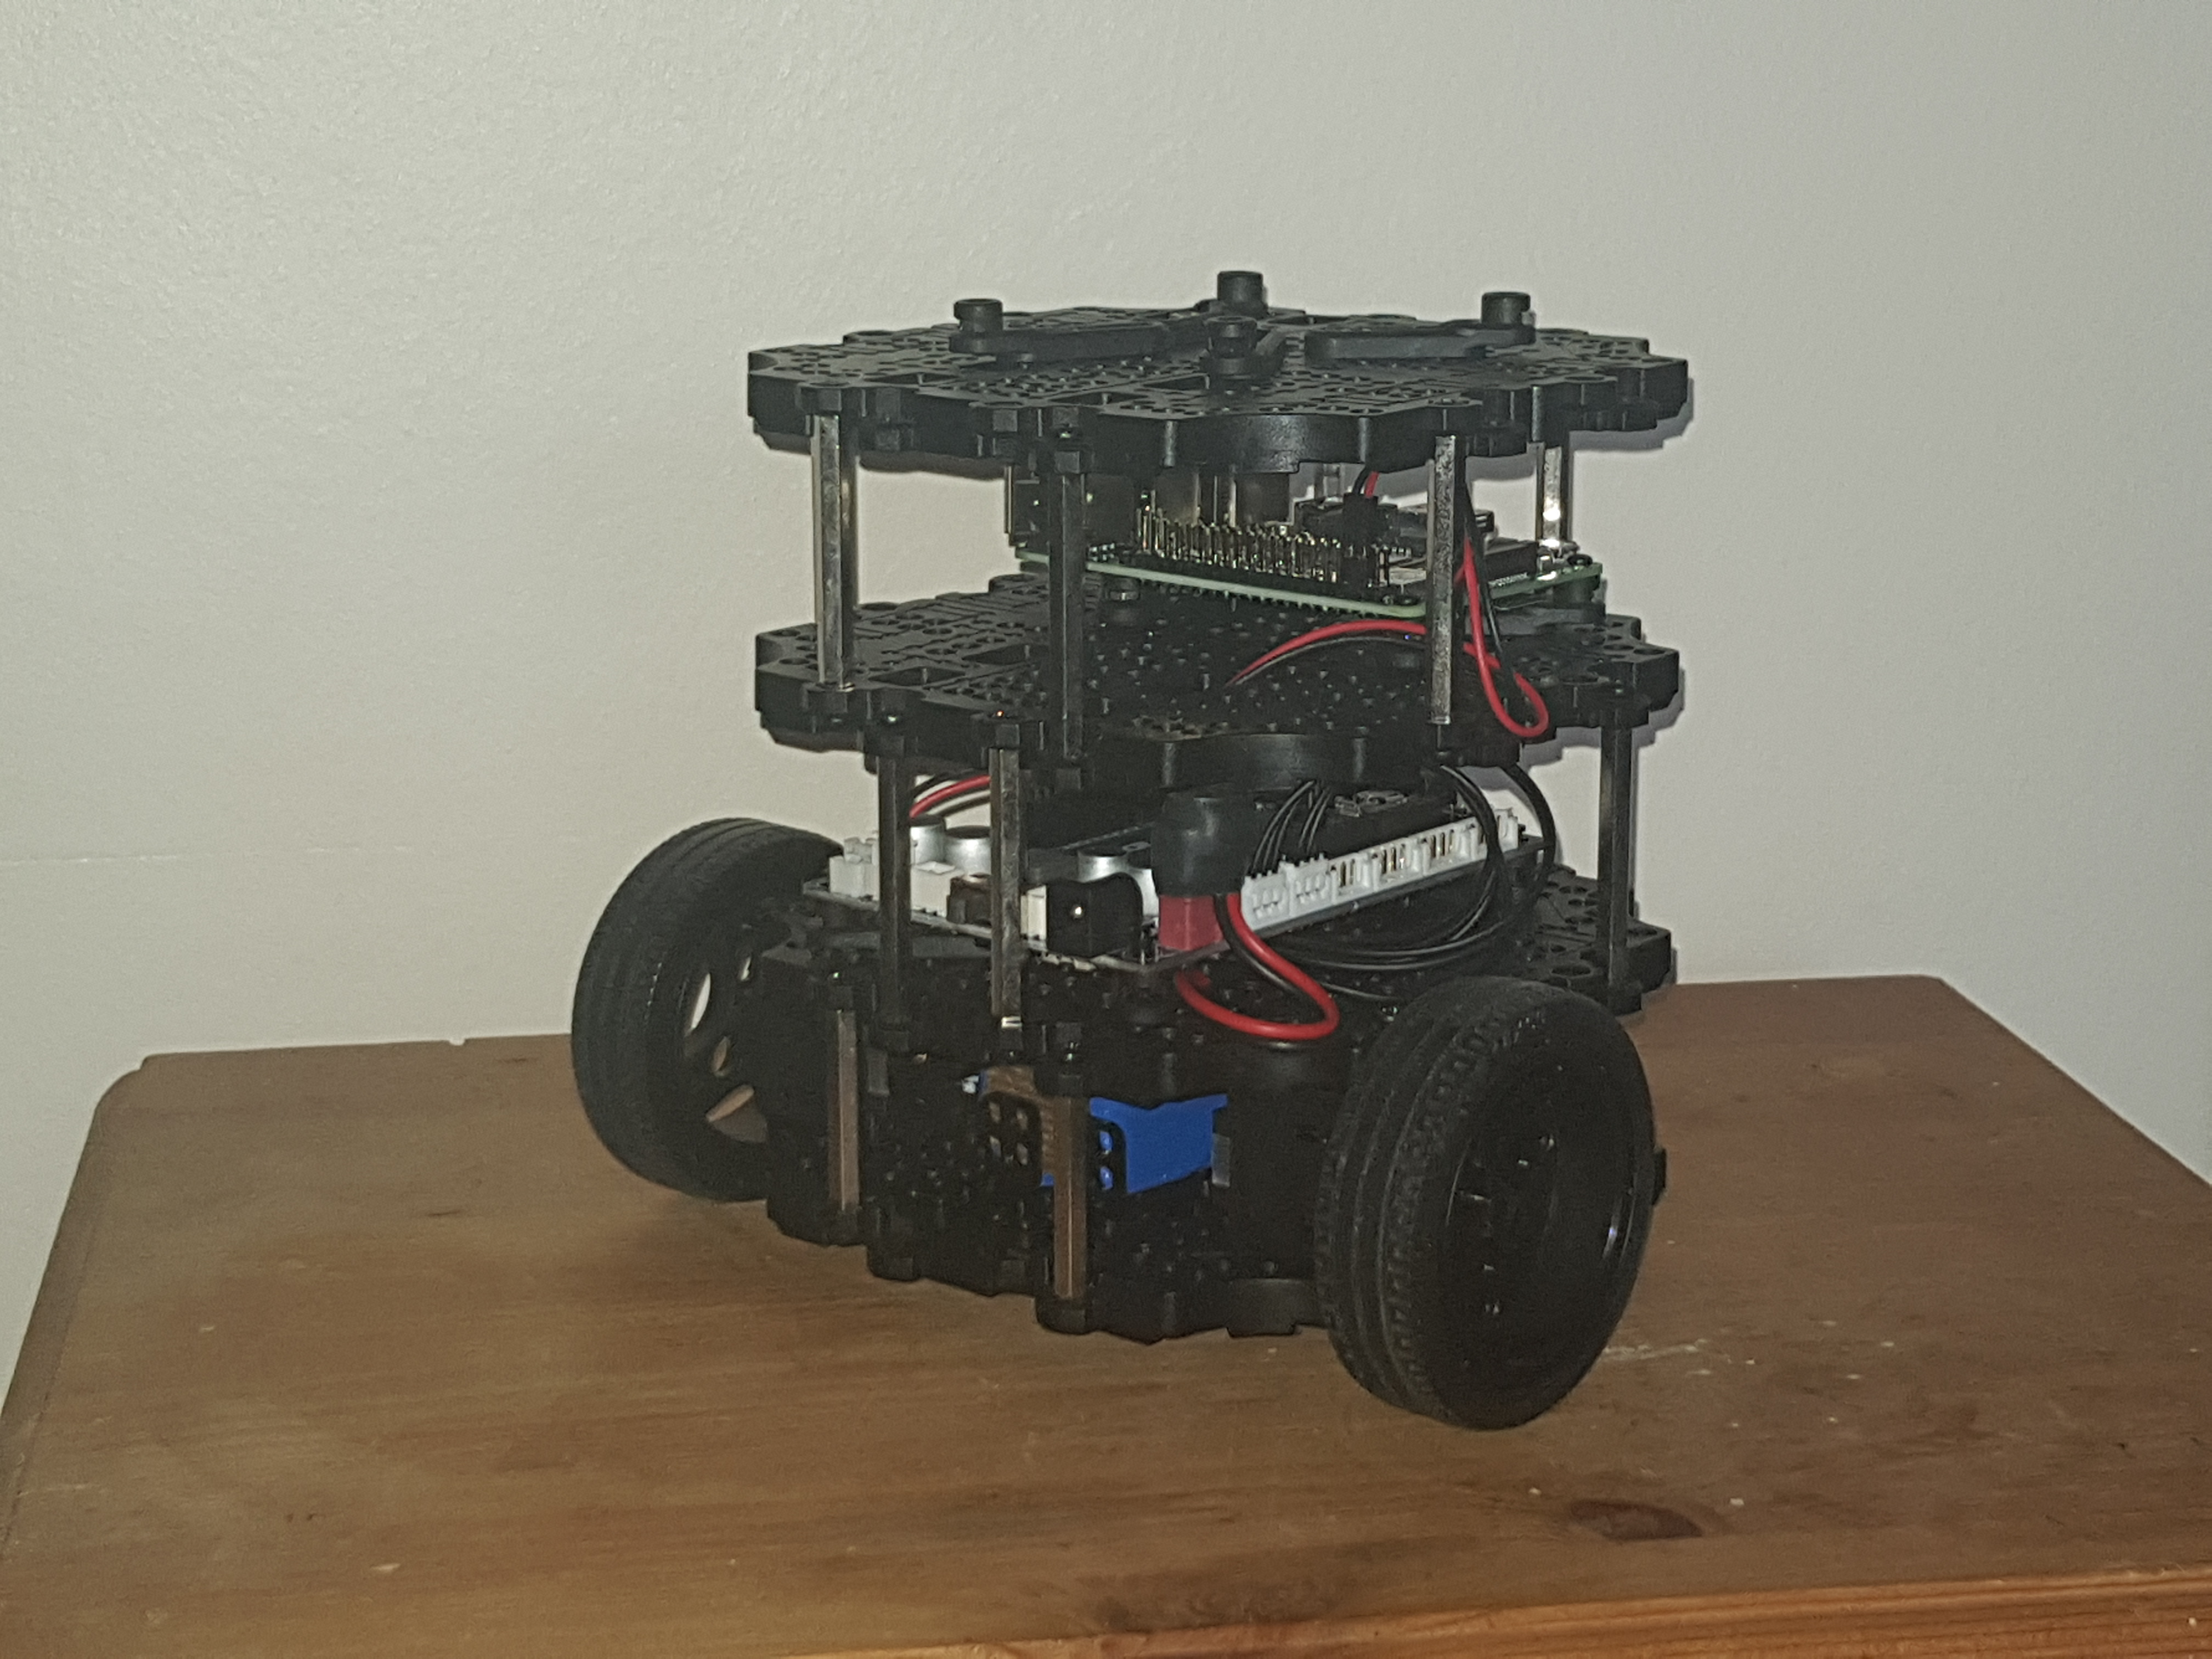
\includegraphics[scale=0.05]{BuiltRobot} \\
			The Turtlebot3 is a ``ROS standard platform robot"\cite{robotis_emanual} which means it is built and setup to use the ROS system, which is outlined further below.
		\subsection*{Hardware}
			The TurtleBot3 version being used is described as ``Burger" and has dimensions of 138mm x 178mm x 192mm (L x W x H). Making it quite small, the main onboard computer is a Raspberry Pi 3 Model B+ which acts as the platform for ROS to run off. The ``BurgerBot" as I'm referring to it, is driven by two Dynamixel motors which provide odometry data back to the system and allow for a maximum translational velocity of 0.22m/s.\cite{turtlebot3_specs} \\
			To interface between the sensors and the Pi, an OpenCR1.0 sits on the second layer of the bot, connecting the battery and dynamixel motors to the Pi via a Micro-USB B to USB A cable, as well as containing an IMU (Inertial Measurement Unit) whose data is passed along the same cable.\\
			Typically the BurgerBot would make use of a LiDar device, however as it is not at all relevant to the project and drains power, I have removed the LiDar from the BurgerBot I am using. The space it frees up makes mounting a camera to the robot significantly easier. 
		\subsection*{Software}
			The Turtlebot3 is a ROS based robot, and as such makes use of this. Open Source ``nodes" are available for the robot and act as an interface between the user code and the robot hardware, saving me from the difficulty of having to implement low level hardware interactions. However this has not purely been a blessing as explained below.			
	\subsection*{ROS}
		\subsubsection*{Overview of the Robot Operating System}
			The Robot Operating System (ROS) is a meta-operating system that runs on top of a regular operating system. It is designed to be highly modular (though one could at times argue too modular) and typically run in a ``Publisher -> Subscriber" model, a unit of executable is referred to as a node and is typically recommended as a reusable task, for example ``sensor drive, sensor data conversion, obstacle recognition, motor drive, encoder input and navigation"\cite{pyo_ros_en_2017}
		\subsubsection*{My experience with ROS}
			Setting up the ROS system has been a challenge for sure. The system is quite stringent on the operating systems it supports for any particular version, the ROS system has a number of distributions: \\
			\includegraphics[scale=0.5]{RosDistro}\cite{ros_distros} \\
			As well as a second version "ROS2" which itself has a number of distributions: \\
			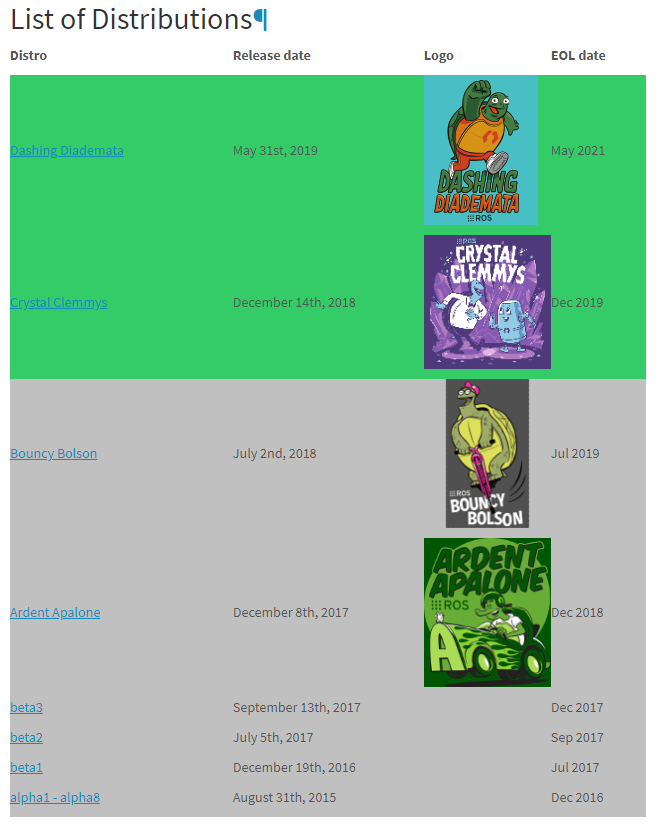
\includegraphics[scale=0.5]{ROS2Distro}\cite{ros2_distros} \\
			This meant I had quite a number of options in how I installed this. \\
			The TurtleBot3 provides software nodes for topic publishing and subscribing, however these are only implemented on certain distros: \\
			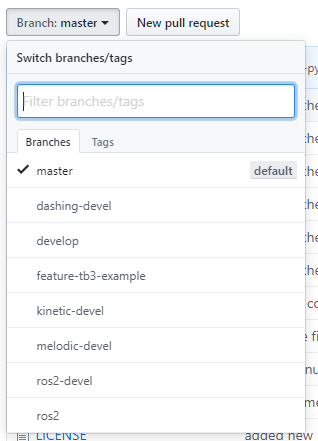
\includegraphics[scale=0.75]{TurtleBot3SupportedDistributions} \\
			As this shows, the turtlebot3 nodes are implemented on: \\
			\begin{enumerate}
				\item Dashing Diademata (Ros2)
				\item Kinetic Kame (Ros1)
				\item Melodic Morenia (Ros1)
			\end{enumerate}
			This narrowed down my options to 3 viable distributions, two of which were under Ros1, and a single one under ros2. The setup instructions provide clear instructions for Kinetic Kame and Dashing Diademata. So whilst this didn't rule out melodic, Kinetic was the first one I attempted. This proved, problematic. Kinetic Kame only supports ``Wily (Ubuntu 15.10), Xenial (Ubuntu 16.04) and Jessie (Debian 8)"\cite{Kinetic_install} which wasn't amazingly helpful as the spare laptop I have with an Ubuntu installation uses Bionic and I wasn't keen to push a second Ubuntu version onto the machine due to the likelihood of conflicts. \\
			This therefore resulted in an attempt to install Melodic Morenia, this proved problematic on the part of the TurtleBot as installing an operating system onto the robot that was supported proved mildly problematic, and though Ubuntu Server 18.0.4 allowed for ROS installation, I found the process particularly difficult and fraught with errors. \\
			This left me with attempting ROS 2 installation with Dashing Diademata, this actually worked. Once again using Ubuntu Server 18.0.4 for the robot, and my Ubuntu Bionic installation on the laptop. I was able to get the system running, connected and run the built in programs. There were a few issues along the way, but those were ironed out eventually. \\
			The next step came in setting up the camera, the department kindly provided a pair of Raspberry Pi V2 Cameras which I had a bracket 3d printed and then attempted to get them setup...Ubuntu Server 18.0.4 is not Raspberry Pi native and setting up the cameras proved nigh on impossible, along this process I broke the operating system several times. So many in fact, that I eventually wrote a script to perform the install procedure on the robot (See appendix 1.) this sped up the process of setting the robot back up again when I broke the software setup.
		\subsection*{USB Camera}
			Eventually abandoning the idea of using the Raspberry Pi camera, I borrowed and have since acquired a Logitech C920 USB camera with which I have written a simple preliminary program to track an object moving around the screen, this served as a test for the camera settings and to refamiliarise myself with the OpenCV libraries (Open (source) Computer Vision)  which is a massively popular and well supported Computer Vision library, extremely popular for research due to how powerful it is. It's not necessarily the most efficient library, but it is very powerful and should suit my purposes nicely. I have a small amount of experience in using an old version of this library and this thankfully has made the beginning configurations and test programs to be significantly easier. \\
			The program simply displays a set of HSV sliders, and given a small bit of configuration to track a particular object, then draws a line as the object is moved around within frame. This program is simply running on a base computer and though it prefers the Logitech C920, functions with any integrated camera. \\
			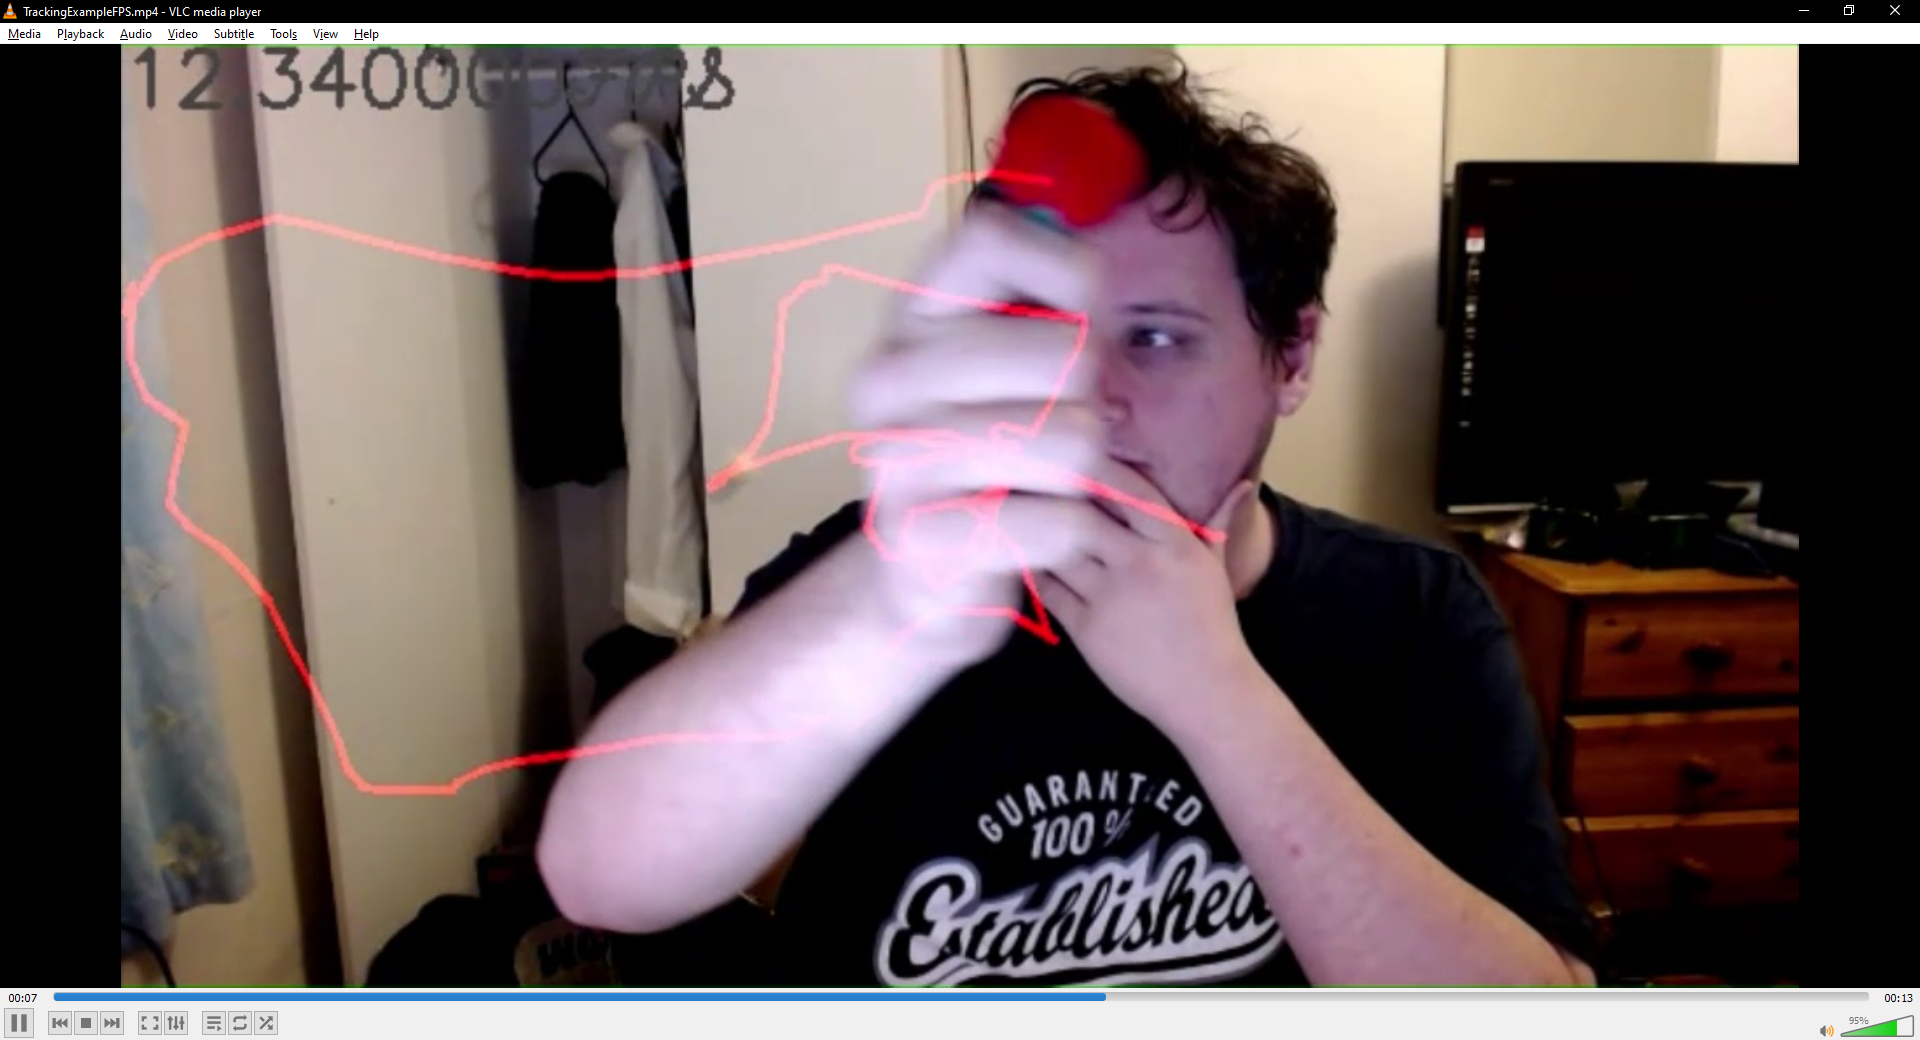
\includegraphics[scale=0.25]{TrackingExampleScreenshot} \\
			Though this program is simple, it employs a number of the basic concepts that the final solution shall have to incorporate, such as thresh-holding, using moments of an image to find the size and location of an object within the frame and blurring to reduce noise. 
		\subsection*{Reflection on Timetable and Progress so far}
			The original timetable suggested that from Week 4 to Week 7, the focus would be on the Calibration/Familiarity goals, and by week 8, the work would shift to the progress report with an understanding that the coursework deadlines would make that tricky. Overall I feel that the timetable has been relatively well kept to, however the difficulties with ROS have meant that the majority of the calibration goals cannot be said to be complete. Though I have code that reacts to the visual stimulus, it hasn't been tied to the robot yet and as such the robots movement and the camera recognition are strongly decoupled currently. \\
			\subsubsection*{Revising the timetable}
				To improve the timetable, some amount of the calibration goals should be done over the Christmas holidays, as well as starting to lean into the progress goals. However given these small adjustments, I believe the original timetable can be mostly kept to. But given the cope of the work, I expect that Progress goals 1, 2 and 3 will take the majority of the time and 4 and 5 will then be an extension on this. Nor necessarily completed in that order. 
			\subsubsection*{Objectives:}
				\section{Calibration/Familiarity Goals}
					\begin{enumerate}
						\item Move the robot in a square.
						\item Move the robot in a predefined fashion in response to a visual stimulus 
						\begin{enumerate}
							\item  Move back and forth when a Red object is visible
							\item Move towards a Red Object
						\end{enumerate}
						\item Recognise small Brightly coloured obstacles
						\begin{enumerate}
							\item Differentiate an obstacle from a goal
						\end{enumerate}
					\end{enumerate}
				
				\section{Progress Goals}
				\begin{enumerate}
					\item Move the object in a way that follows a goal and avoids obstacles
					\item Recognise larger flat obstacles 
					\begin{enumerate}
						\item Attempt to avoid flat obstacles whilst moving
					\end{enumerate}
					\item Make predictions on the location of the goal object in relation to the position
					\item Manoeuvre around a more complex set of obstacles given knowledge of the goal
					\item Search for the goal object in an unknown environment avoiding obstacles.
				\end{enumerate}
			
				\section{Stretch Goals}
				\begin{enumerate}
					\item Use background distinguishing features to aid dead-reckoning of location
					\item Avoid varied obstacles e.g.
					\begin{enumerate}
						\item Posts
						\item Cylinders
						\item Arbitrary non-goal objects
					\end{enumerate}
					\item Identify multiple goal objects and their separate locations, mapping between them
				\end{enumerate}
				
\section*{Future plans}
	\subsection*{Experiments}
		To test the effectiveness of the solution in a reasonably scientific way, a controlled environment is necessary. I'd like to create a simple maze environment for the robot to manoeuvre around. A number of arrangements for the maze can be generated. From this we can measure a number of parameters relating to the performance in moving through the environment. \\
		The format for the experiments will be thus: \\
		The robot will start on the edge of the environment facing towards the maze and from there attempt to find a red cube similar to this one: \\
		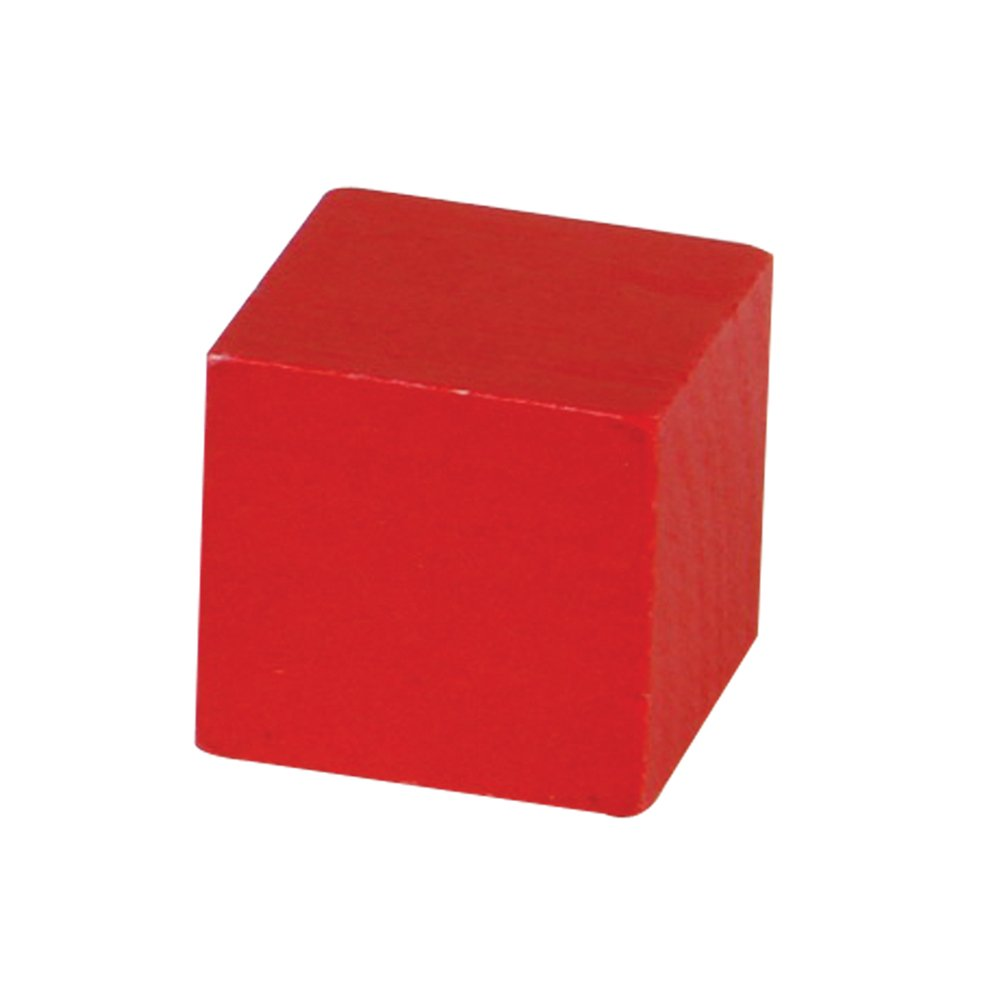
\includegraphics[scale=0.2]{RedCube}  \\
		This is simply to give the robot a reasonable chance of entering the environment and not immediately moving away from the environment which may result in a ``cheating" solution of going around the environment to find the target. \\
		The maze will contain some number of obstacles which may or may not block line of sight. \\
		To test objective 1, the obstacles will not block line of sight and will present a clear path towards the goal, allowing the robot to hypothetically move straight to the goal ideally. \\
		to test objective 2, non-line-of-sight-blocking obstacles which are distinguishable from their environment can make up the obstacles, given their distinguish-ability and lack of line of sight blocking, the robot is able to focus on avoidance, keeping an "eye" on the goal, rather than having to focus on mapping. \\
		To test objective 3, more varied obstacles which may or may not block line of sight, the robot will have to demonstrate an ability to map and explore in order to successfully reach the goal without just blind luck.
		Testing objective 4 will be difficult to do in a measurable way, a reasonable experiment is to compare pose estimates without camera use and with the camera, against the correct values, this can then be compared numerically to see the level of improvement made. 
		For a given maze configuration these things can be measured about the maze:
		\begin{enumerate}
			\item Length of ideal route
			\item Number of obstacles in maze
			\item Size of maze
			\item Complexity of route as a measure of turns required to reach goal.
		\end{enumerate}
		Using this data to give a comparison between maze layouts, we can then measure a number of elements about the performance of a robot in this environment, such as:
		\begin{enumerate}
			\item Time to goal
			\item Obstacle collisions
			\item Wrong turns
			\item Battery power used
		\end{enumerate}
		These measurements can then provide comparisons between different stages of implementation. To provide a baseline, it may be worth implementing a simple ``Remote Control" program for the robot which provides a camera feed and simple control scheme to provide a benchmark against which the algorithm can be measured. This may also provide some aid in identifying bugs or issues in the setup.
	
	\subsection*{Resources to be used/acquired}
		These experiments will require a few resources to execute, thought they shouldn't be too difficult to acquire. 
		\begin{enumerate}
			\item Red cube
			\item Obstacles of small height, e.g. Non-red blocks
			\item Obstacles of robot-comparable height (Approx. 20cm)
		\end{enumerate}
		I am currently attempting to acquire the first two sets of items from an old toy left at home; this is proving only mildly difficult in terms of scheduling and distance. The third set of items I have yet to have any particularly good ideas for, although A4 sized folders (31cm x 28cm) are typically capable of standing on their own and would be a good height for this, as well as being generally cheap to buy if necessary, or I may be able to borrow enough.
		
	\subsection*{Implementation steps to take}
		The system is effectively split into two major parts: Vision analysis and robot control. Separately these two parts have progress to be made as well as integration to be done between them. A significant step is the use of a node for the ROS operating system made by another developer under the github handle ``klintan": (https://github.com/klintan/ros2\_usb\_camera) This node will hopefully enable some of the integration to be smoother by providing a cross point between the camera feed and the robot operating system. This saves the effort of having to implement such functionality manually thankfully. \\
		With this node in place, the live camera feed can be published to the controlling computer for processing and saving. Maintaining the robot - computer control balance seems to be in the spirit of ROS and enables greater processing power at the cost of latency which, given the robot’s maximum speed being fairly low, should hopefully not be problematic.
		\subsubsection*{Possible future stumbling blocks}
			This project like any other is not without some risks. The ROS system is genuinely a little bit frustrating but, given the progress that has been made so far, the project should have gotten over the largest hurdle of using the system. However, I cannot discount the possibility that some element of the system or understanding of its processes may cause a delay in the project. \\
			In regards to the computer vision, many of the algorithms that can be used to aid in this process are computationally expensive and reduce the effective update rate of the robot. Whilst millisecond by millisecond updates are not required, if the computation grows complex enough, there may be issues with the effective update rate growing too slow to move the robot at more than a snail's pace. Hopefully this can be mitigated with reduced resolutions and optimisation to the algorithm itself which may prove to be a benefit in improving the overall quality of the algorithm developed. \\
			There is a risk of the hardware failing in some way. The hardware has been very reliable thus far in the project and as such I do not consider this a particularly likely risk. Hardware projects have a habit of presenting various issues that distract from the main problem of the project. 
	\subsection*{Considerations for the presentation}
		Presenting this project should hopefully be quite interesting as far as demonstrations go. Two main methods of demonstrating come to mind: \\
		\begin{itemize}
			\item Live demonstration of maze solving with camera feed.
			\item Annotated video of robot solving the maze from camera feed showing identifications of obstacles and goal.
		\end{itemize}
		Having these two options gives a bit of leeway on how to present the project as the live demonstration may not necessarily be feasible given time and space constraints. However the annotated video should provide a reasonable backup that continues to be fairly interesting and show the capabilities of the project effectively. \\
		An ideal annotated video would show the robot moving through an environment with nicely drawn lines indicating belief in obstacle locations and approximate angles/distances away. This would give a frame by frame demonstration of the robot's capabilities in understanding its environment.
	

\appendix
\section*{TurtleBotRos2SetupScript.sh}
\begin{lstlisting}[language=BASH]
	sudo apt-get update
	yes | sudo apt-get install cmake g++
	echo "git, cmake and g++ install"
	
	sudo swapoff -a
	sudo fallocate -l 1G /swapfile
	sudo chmod 600 /swapfile
	sudo mkswap /swapfile
	sudo swapon /swapfile
	sudo bash -s 'echo "/swapfile swap swap defaults 0 0" >> /etc/fstab'
	
	sudo locale-gen en_US en_US.UTF-8
	sudo update-locale LC_ALL=en_US.UTF-8 LANG=en_US.UTF-8
	export LANG=en_US.UTF-8
	
	sudo apt-get update
	echo "Update done"
	yes | sudo apt-get install curl gnupg2 lsb-release
	echo "Curl, gnupg2, lsb-release installed"
	curl -s https://raw.githubusercontent.com/ros/rosdistro/master/ros.asc | sudo apt-key add -
	
	sudo sh -c 'echo "deb [arch=amd64,arm64] http://packages.ros.org/ros2/ubuntu `lsb_release -cs` main" > /etc/apt/sources.list.d/ros2-latest.list'
	
	sudo apt-get update
	echo "Re-update"
	yes | sudo apt-get dist-upgrade
	echo "Dist-upgrade complete"
	yes | sudo apt-get install ros-dashing-ros-base
	echo "Ros2 installed"
	
	source /opt/ros/dashing/setup.bash
	echo "source /opt/ros/dashing/setup.bash" >> ~/.bashrc
	
	yes | sudo apt-get install python3-argcomplete python3-colcon-common-extensions libboost-system-dev
	echo "apt-get complete"
	mkdir -p ~/turtlebot3_ws/src && cd ~/turtlebot3_ws/src
	git clone -b ros2 https://github.com/ROBOTIS-GIT/hls_lfcd_lds_driver.git
	git clone -b ros2 https://github.com/ROBOTIS-GIT/turtlebot3_msgs.git
	git clone -b ros2 https://github.com/ROBOTIS-GIT/turtlebot3.git
	git clone -b ros2 https://github.com/ROBOTIS-GIT/DynamixelSDK.git
	
	cd ~/turtlebot3_ws/src/turtlebot3
	rm -r turtlebot3_cartographer turtlebot3_navigation2
	cd ~/turtlebot3_ws/
	source /opt/ros/dashing/setup.bash
	colcon build --symlink-install --parallel-workers 1
	echo "turtlebot3_ws built"
	
	echo 'export TURTLEBOT3_MODEL=burger' >> ~/.bashrc
	echo 'source ~/turtlebot3_ws/install/setup.bash' >> ~/.bashrc
	echo 'export ROS_DOMAIN_ID=42 #TURTLEBOT3' >> ~/.bashrc
	source ~/.bashrc
	
	cd ~/turtlebot3_ws/src/turtlebot3/turtlebot3_bringup
	sudo cp ./99-turtlebot3-cdc.rules /etc/udev/rules.d/
	sudo udevadm control --reload-rules
	sudo udevadm trigger
	
	sudo dpkg --add-architecture armhf
	sudo apt-get update
	echo "updated again"
	yes | sudo apt-get install libc6:armhf
	echo "libc6 installed"
	
	cd && rm -rf opencr_update.tar.bz2
	wget https://github.com/ROBOTIS-GIT/OpenCR-Binaries/raw/master/turtlebot3/ROS2/latest/opencr_update.tar.bz2
	tar -xjf ./opencr_update.tar.bz2
	
	export OPENCR_PORT=/dev/ttyACM0
	export OPENCR_MODEL=burger
	cd ~/opencr_update && ./update.sh $OPENCR_PORT $OPENCR_MODEL.opencr
\end{lstlisting}

\nocite{*}
\bibliographystyle{acm}
\bibliography{ProgressReport}

\end{document}